\documentclass[fleqn,14pt]{wlscirep}
\usepackage[utf8]{inputenc}
\usepackage[T1]{fontenc}
\usepackage{amsthm}
\usepackage{amsmath}
\newtheorem{lemma}{Lemma}
\newtheorem{sublemma}{Lemma}[lemma]
\title{Point spread functions and aureoles}

\author[1,*]{Peter Thejll}
%\author[2]{Bob Author}
%\author[1,2,+]{Christine Author}
%\author[2,+]{Derek Author}
\affil[1]{Danish Meteorological Institute, Climate Research, Copenhagen Ø, DK-2100, Denmark}
%\affil[2]{Affiliation, department, city, postcode, country}

\affil[*]{pth@dmi.dk}

%\affil[+]{these authors contributed equally to this work}

%\keywords{Keyword1, Keyword2, Keyword3}

\begin{abstract}
A realistic point spread function is used to convolve delta-functions and one- and two-dimensional objects, yielding approximate halos or 'aureoles'.
\end{abstract}
\begin{document}

\flushbottom
\maketitle
% * <john.hammersley@gmail.com> 2015-02-09T12:07:31.197Z:
%
%  Click the title above to edit the author information and abstract
%
\thispagestyle{empty}

%\noindent Please note: Abbreviations should be %introduced at the first mention in the main text – no %abbreviations lists. Suggested structure of main text %(not enforced) is provided below.

\section*{Introduction}

In optics, a point spread function (PSF) describes how the light from a point source is scattered by the act of observation. More complex sources can be built from weighted delta-functions, and we want to understand how light is scattered around such composite sources by considering simple examples. We shall call the light scattered around a composite source its halo or aureole.

\section*{Method}

Let a point source be given by a Dirac $\delta$-function at position $r_0$. Viewing that source through an optical system with an intrinsic PSF then yields an image of the source, but now convolved by the PSF:
\begin{eqnarray}
PSF(r)*\delta(r-r_0) = PSF(r_0).
\end{eqnarray}
A composite source can we written as a sum of weighted $\delta$-functions:

\begin{eqnarray}
O(r) = \sum w_i \cdot \delta(r-r_i),
\end{eqnarray}
where the $w_i$ could be e.g. pixel-intensities in an image-array.

Viewing such a composite object $O(r)$ leads to an image $I$ which is a convolution:
\begin{eqnarray}
I(r) = PSF(r)*O(r) = PSF(r)*\sum w_i \cdot \delta(r-r_i) = \sum w_i \cdot PSF(r)*\delta(r-r_i) = \sum w_i \cdot PSF(r_i).
\end{eqnarray}
We recast this slightly and make the weights a spatially-dependent function. We also go to one-dimensional images.
Let the object intensity $O$ be a Heaviside step-function $H$:
 
\begin{equation*}
    H(x) = \begin{cases}
               1 & \text{for x}$<$0\\
               0 & \text{elsewhere}.
           \end{cases}
\end{equation*}

The convolution is then
\begin{eqnarray}
I(X) = PSF(x)*H(x) = \int_{-\infty}^{0} PSF(x-x') dx'
\end{eqnarray}
Let us now do this integral for a radially symmetric 'power-law' PSF, which is empirically inspired:
\begin{equation*}
    PSF(x) = \begin{cases}
               1/x^a        & \text{for x}$>$\epsilon\\
               1/\epsilon^a & \text{elsewhere}.
           \end{cases}
\end{equation*}
The above gives us, for $x<-\epsilon$:
\begin{eqnarray}
I(x) = \int_{-\infty}^{0} \frac{1}{|x-x'|^a} dx' = \int_{-\infty}^{x-\epsilon} \frac{1}{(x'-x)^a} dx' + \frac{2\epsilon}{\epsilon^a} + \int_{x+\epsilon}^{0} \frac{1}{(x-x')^a} dx',
\end{eqnarray}
which after some manipulation yields
\begin{eqnarray}
I(X) = \frac{2\epsilon}{\epsilon^a} + \frac{1}{(a-1)(x^{a-1})}.
\end{eqnarray}
Likewise, for $x>\epsilon$ we get:
\begin{eqnarray}
I(x) = \int_{-\infty}^{0} \frac{1}{|x-x'|^a} dx' = \frac{1}{(a-1)(x^{a-1})}.
\end{eqnarray}
We shall ignore the case $|x| \leq \epsilon$.

For this one-dimensional case we see that the exponent of the inverse power-law that describes the slope of the halo or aureole is 1 less than the slope of the PSF itself. This is for a semi-infinite uniform object $O$, of course.



\subsection*{Subsection}

Example text under a subsection. Bulleted lists may be used where appropriate, e.g.

\begin{itemize}
\item First item
\item Second item
\end{itemize}

\subsubsection*{Third-level section}
 
Topical subheadings are allowed.

\section*{Discussion}

The Discussion should be succinct and must not contain subheadings.

\section*{Methods}

Topical subheadings are allowed. Authors must ensure that their Methods section includes adequate experimental and characterization data necessary for others in the field to reproduce their work.

\bibliography{sample}

\noindent LaTeX formats citations and references automatically using the bibliography records in your .bib file, which you can edit via the project menu. Use the cite command for an inline citation, e.g.  \cite{Hao:gidmaps:2014}.

For data citations of datasets uploaded to e.g. \emph{figshare}, please use the \verb|howpublished| option in the bib entry to specify the platform and the link, as in the \verb|Hao:gidmaps:2014| example in the sample bibliography file.

\section*{Acknowledgements (not compulsory)}

Acknowledgements should be brief, and should not include thanks to anonymous referees and editors, or effusive comments. Grant or contribution numbers may be acknowledged.

\section*{Author contributions statement}

Must include all authors, identified by initials, for example:
A.A. conceived the experiment(s),  A.A. and B.A. conducted the experiment(s), C.A. and D.A. analysed the results.  All authors reviewed the manuscript. 

\section*{Additional information}

To include, in this order: \textbf{Accession codes} (where applicable); \textbf{Competing interests} (mandatory statement). 

The corresponding author is responsible for submitting a \href{http://www.nature.com/srep/policies/index.html#competing}{competing interests statement} on behalf of all authors of the paper. This statement must be included in the submitted article file.

\begin{figure}[ht]
\centering
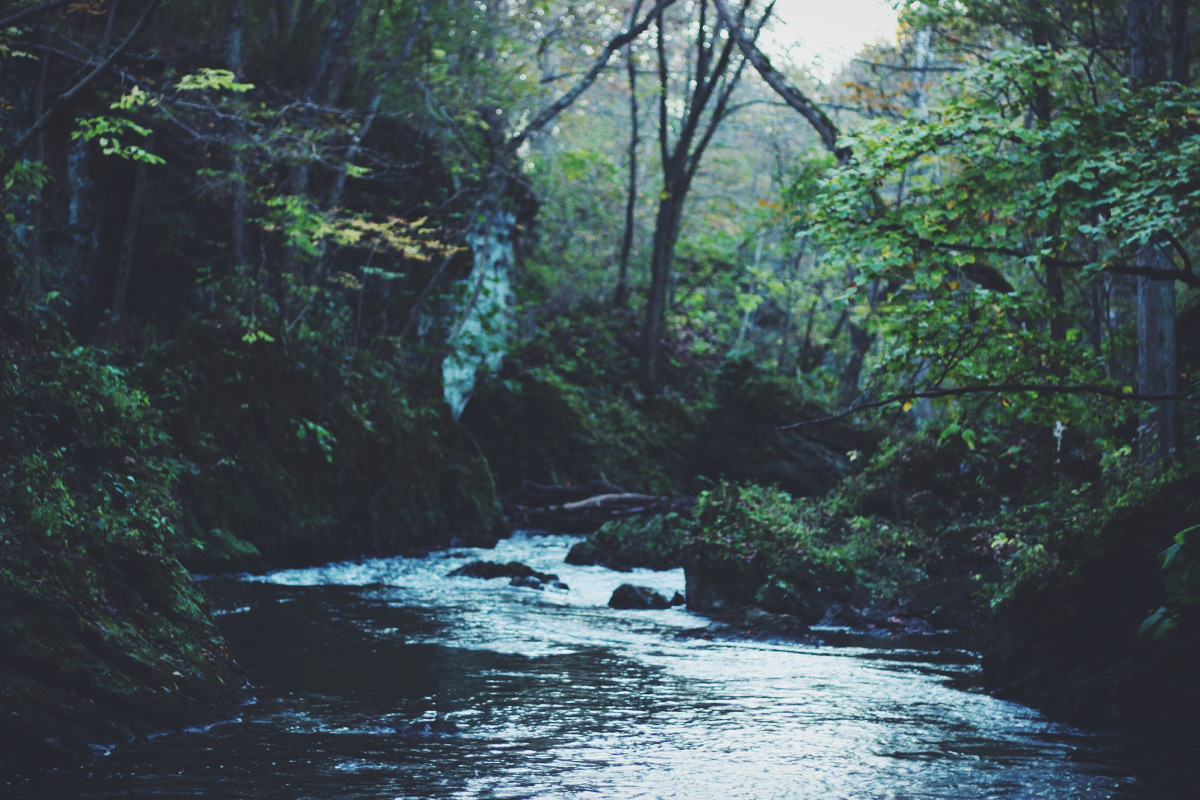
\includegraphics[width=\linewidth]{stream}
\caption{Legend (350 words max). Example legend text.}
\label{fig:stream}
\end{figure}

\begin{table}[ht]
\centering
\begin{tabular}{|l|l|l|}
\hline
Condition & n & p \\
\hline
A & 5 & 0.1 \\
\hline
B & 10 & 0.01 \\
\hline
\end{tabular}
\caption{\label{tab:example}Legend (350 words max). Example legend text.}
\end{table}

Figures and tables can be referenced in LaTeX using the ref command, e.g. Figure \ref{fig:stream} and Table \ref{tab:example}.

\end{document}